Designing easily extensible and testable numerical codes is inherently challenging,
the complexity of numerical algorithms and the continuous nature of their results
make it hard to separate the logic from application specific implementation details.
As \gls{PyExaFMM} is implemented in Python, an \gls{interpreted} and inherently
\gls{object-oriented-language}, we are able to
use some common and powerful object oriented design principles to ensure extensibility
and testability. However, as most parallel optimisation software relies on access to data
containers themselves, rather than an abstraction layer between a data object
and a client object, the number of object abstractions must also be kept to a
minimum.

Concerns about the overhead of using the object oriented design principles, in comparison to directly manipulating
primitives, such as those available in compiled languages such as C
or C++, are misplaced for two reasons. Firstly, the implementation of Python objects
is syntactic sugar, methods and data for a given object are written into
a simple dictionary structure at run time, with the `class' syntax common to other
object oriented languages such as C++ or Java, offered as they are familiar to
the programmer coming from such languages. Furthermore, all `primitives' such as
integers and strings in Python are actually objects by design, being quite different
in their construction from C or C++ where the programmer is given the power to
allocate memory for true primitives themselves. In Python the overhead therefore
comes from the interpreter, which transforms the source code into byte code which
is then compiled. This additional interpreter layer is the source of Pythonic overhead,
rather than the object abstraction in itself. Therefore, once the decision has
been made to use Python, there isn't a significant overhead from using object
oriented design principles, with the added benefit of increasing programmer
productivity, and increasing testability \cite{Ramalho:2015:Oreilly}. Secondly,
the vast Python ecosystem of optimised libraries for numerical computation allow
for the manipulation and allocation of primitives in memory in a manner closer to a compiled language.
Specifically, \gls{PyExaFMM} implements all of its containers with NumPy, which
offers an interface for the allocation and access of numerical data with C-like
efficiency, due to the underlying subroutines being written in C. Additionally,
\gls{PyExaFMM} uses just-in-time (\gls{JIT}) via the Numba library on
numeric subroutines implemented with NumPy containers. Just-in-time compilation
refers to a system which analyses the byte-code generated by an interpreter
for repetitive operations which would benefit from compilation and caching, therefore
combining the speed benefits of compiled languages, with the flexibility of interpreted
languages.

\begin{figure}
    \centering
    {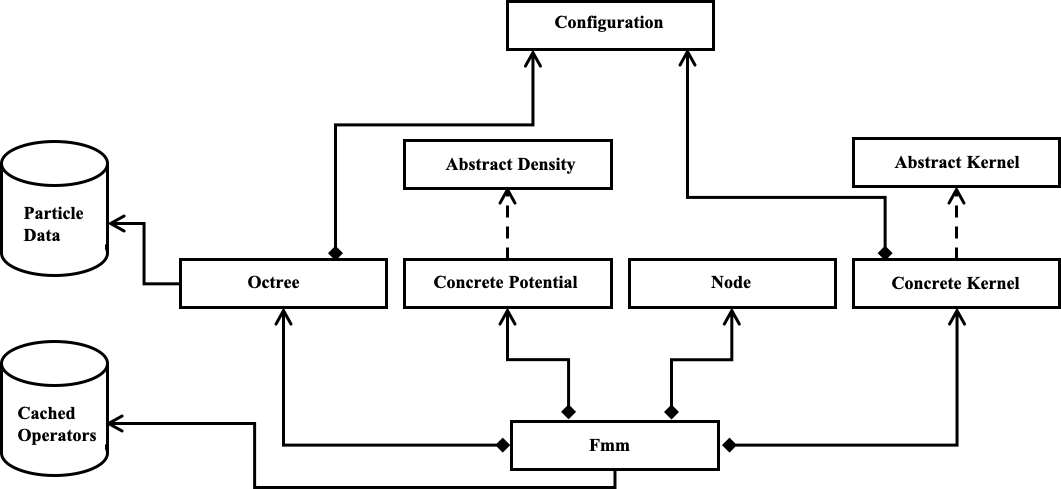
\includegraphics[width=\textwidth]{chapter2/object_organisation.png}}
    \vspace{0pt}
    \caption{Object hierarchy of \gls{PyExaFMM}. Objects are illustrated with
    square boxes, and data (either on disk, or in a cache) by a cylinder using
    standard software engineering convention \cite{Gamma:1994:Addison}. Solid
    lines indicate a dependent relationship, whereas dashed lines
    indicate an inheritance relationship. A diamond arrow head indicates an
    object instantiation, a pointed arrow head indicates the direction of a
    dependency.}
    \label{fig:2_5_architecture}
\end{figure}

\begin{figure}
    \centering
    {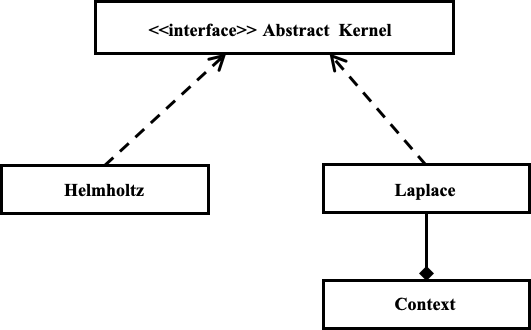
\includegraphics[width=0.6\textwidth]{chapter2/kernel_strategy.png}}
    \vspace{0pt}
    \caption{Strategy design pattern implemented for the Kernel class.  Solid
    lines indicate a dependent, relationship dashed lines
    indicate an inheritance relationship. A diamond arrow head indicates an
    object instantiation, a pointed arrow head indicates the direction of a
    dependency.}
    \label{fig:2_5_strategy_kernel}
\end{figure}

The main object hierarchy used in \gls{PyExaFMM} is shown in figure
(\ref{fig:2_5_architecture}). The first major design principle followed is dependency
inversion, whereby components are arranged in a hierarchy such that downstream
components, whether they be objects or entire modules, are not dependent on
upstream components for any of their logic. Instead, they are coupled together via
abstractions in the form of known interfaces \cite{Gamma:1994:Addison}. \gls{PyExaFMM} is architected
around the main `Fmm' object, which is placed downstream, at the top of the object hierarchy.
This object contains methods that implement the logic for the
upward and downward pass steps of the \gls{FMM} loop, as well as access methods
for the source and target particle data, and the results of the expansion at each box, for each level of the associated octree.
In \gls{PyExaFMM}, a configuration object, specified via a \textbf{\gls{JSON}} file, is instantiated
at runtime. This is used to instantiate an Fmm object with its upstream dependencies.
Namely, an Octree object is configured, which creates a linear octree as well
as the \gls{JIT} compiled bitwise methods for tree traversal, from user
specified source and target particle data. Additionally, a user specified kernel choice
from the configuration file is used to instantiate a kernel object.
This kernel object is defined using the strategy design pattern
\cite{Gamma:1994:Addison}, illustrated in figure (\ref{fig:2_5_strategy_kernel}).
This pattern allows for concrete implementations of kernel objects to be separated
from the context in which they're used, allowing the user - in this case the
Fmm object - to access kernel functions via a uniform interface. Kernel
objects also allow for the encapsulation of
kernel specific information such as their scaling properties at different levels
of an octree. Furthermore, the precomputed operator matrices are loaded from a cache,
and injected into the Fmm object. Crucially, this means that the Fmm object can
remain ignorant of the implementation details of how these operators were computed.

The main point to note is that a loose hierarchy of objects allows for
the logic of the main \gls{FMM} loop to be separated from the code it depends on
, for example for the creation and partitioning of an octree.
Safe interactions between objects, further enforced by interfaces for data.
Specifically the Abstract Density and Node classes define interfaces for access to concrete Potential density
objects (used to store the potential computed at a target particle as a result
of the FMM algorithm), and the multipole or local expansions for a given box in an octree respectively,
as well as their underlying Numpy containers, in a uniform manner.
These types of objects are often referred to as return objects in object-oriented
design as they enforce the format of the result of a computation,
here they help offer guarantees to their client, the main Fmm object,
about the dimensions and data types of their respective containers.

The second major design principle followed by \gls{PyExaFMM} is
the separation of concerns, whereby implementation details of distinct
components of a program are separated by modules, with known interfaces
\cite{Gamma:1994:Addison}. Specifically, \gls{PyExaFMM} separates into independent
scripts: the code for operator caching discussed in Section \ref{sec:2_3_operator_caching},
and the code for SVD based compression of the M2L operator matrices discussed in
Section \ref{sec:2_4_svd_compression}. These scripts are accessible via the
command-line, through a custom command-line interface, invoked with the command
prefix `ci', created as a part of \gls{PyExaFMM} package. We defer to the \gls{PyExaFMM}
documentation for more information about the command-line interface, however a
basic workflow would start at the command line, creating the \gls{M2M}
\gls{L2L} and \gls{M2L} operator matrices, and compressing the \gls{M2L} matrices,

\begin{verbatim}
Last login: <Day> <Month> <Date> 00:00:00 on console
user@Workstation ~ % ci compute-operators
user@Workstation ~ % ci compress-m2l
\end{verbatim}

These commands are again configured using the \gls{JSON} configuration file
which specifies the parameters used in a simulation, such as the order the
multipole and local expansions. Following the execution of the above,
\gls{PyExaFMM} is automatically configured with the required
operator and particle data, and simulations can be run from within a Python
interpreter or as a script using the following syntax,

\begin{python}
from fmm.fmm import Fmm

# Instantiate FMM object
fmm = Fmm(config_filename='my_custom_config.json')

# Run Upward Pass
fmm.upward_pass()

# Run Downward Pass
fmm.downward_pass()

# Get Results at Target Points
fmm.result_data
\end{python}

At runtime, the instantiation of the Fmm object is preceded by the injection of
dependencies from beneath it in the object hierarchy. However, this complexity is
hidden from the user, who only specifies simulation parameters and source
and target particle data locations via a \gls{JSON} configuration file, and interacts
with simulation outputs via the Fmm object's interface.

The utility of separating functionality to do with operator computation, and
compression into separate scripts is that it allows for iterative optimisation
without impacting on the main logic, or design, of \gls{PyExaFMM}. For example,
the main Fmm object is in general ignorant of whether multiprocessing
is being used in operator precomputations, or what the regularisation parameter
was taken to be for computing pseudoinverses of kernel operator matrices
via the SVD has been taken to be, or other specific optimisations outside of the
main loop's logic. This is as it should be, as if the Fmm
object contained too many implementation details it would obfuscate the logic,
making the code harder to debug. This encapsulates the idea of the separation of
concerns.

\gls{PyExaFMM} takes this further by creating modules for specific
operations called by these scripts; specifically it offers its own multiprocessing
and SVD utility modules, which offer wrappers around common interfaces from
underlying standard Python functionality, specialised for usage in \gls{PyExaFMM}.
This offers an advantage in that their implementation can also be changed,
without effecting the logic of the operator computation and compression scripts.
For example, the planned extension to randomised \gls{SVD} methods discussed in
Section \ref{sec:2_4_svd_compression} can be separately implemented in \gls{PyExaFMM}'s
\gls{SVD} utility module while maintaining the wrapper's interface, allowing for the new
functionality to propagate into the operator compression script without
a change of the script's logic. Separation of concerns as a design
principle naturally leads to extensible code \cite{Gamma:1994:Addison}.
